\documentclass[12pt, a4paper]{scrreprt}
\usepackage[margin=2.5cm]{geometry}
\usepackage[hidelinks]{hyperref}
\usepackage{graphicx,xcolor,listings,tikz,enumitem}
\usetikzlibrary{positioning, arrows.meta, shapes, fit}

\definecolor{codegreen}{rgb}{0,0.6,0}
\definecolor{codegray}{rgb}{0.5,0.5,0.5}
\definecolor{codepurple}{rgb}{0.58,0,0.82}
\definecolor{backcolour}{rgb}{0.95,0.95,0.92}

\lstdefinestyle{mystyle}{
  backgroundcolor=\color{backcolour},
  commentstyle=\color{codegreen},
  keywordstyle=\color{blue},
  stringstyle=\color{codepurple},
  basicstyle=\ttfamily\footnotesize,
  numbers=left,
  numbersep=5pt,
  breaklines=true,
  tabsize=2
}
\lstset{style=mystyle}

\newcommand{\faculty}{Faculty Applied Information Technology}
\newcommand{\studies}{Bachelor of Cyber-Security}
\newcommand{\thesistitleDE}{Projekt "WeedDetector" \\ Projektübergabe}
\newcommand{\submissiondate}{05.\ Juli 2025}
\newcommand{\supervisor}{Prof.\ Dr.\ Holger Jehle}

\begin{document}

\begin{titlepage}
  \centering
  {\LARGE Technische Hochschule Deggendorf \\ \faculty \par}
  \vspace{0.3cm}
  {\Large Studiengang \studies \\[1.5cm]}
  {\Huge\bfseries \thesistitleDE\par}
  \vfill
  \begin{minipage}[t]{0.45\textwidth}
    \textbf{Vorgelegt von:}\\
    \\
    Christof Renner (22301943)\\
    Manuel Friedl (1236626)\\
    \\
    \\
    \\
    \\
    Datum: \submissiondate
  \end{minipage}\hfill
  \begin{minipage}[t]{0.45\textwidth}
    \textbf{Prüfungsleitung:}\\
    \\
    \supervisor
  \end{minipage}
\end{titlepage}

\tableofcontents
\newpage

\chapter{Einführung und Projektübersicht}

\section{Motivation und Zielsetzung}

\begin{figure}[h!]
    \centering
    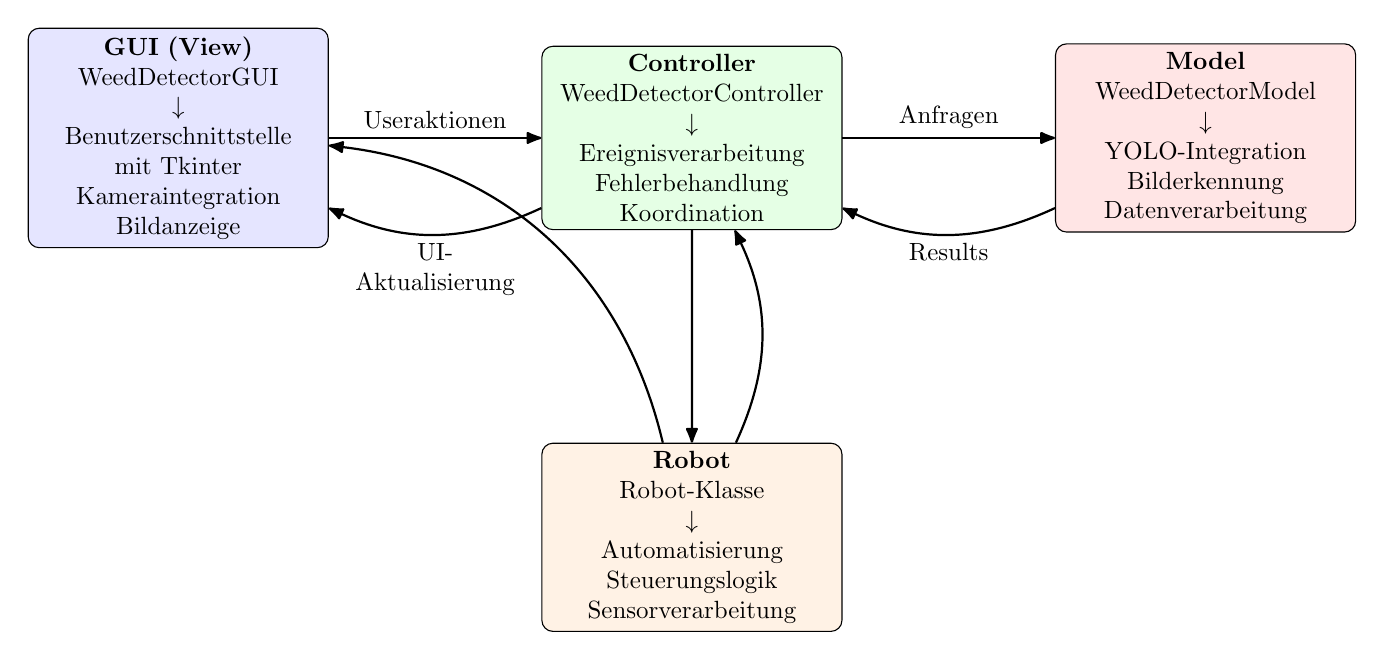
\begin{tikzpicture}[
        scale= 0.9,
        transform shape,
        node distance=3 cm and 3cm,
        box/.style={draw, text width=4cm, align=center, rounded corners, minimum height=2cm},
        arrow/.style={draw, thick, -{Latex[round]}}
    ]

    % Hauptkomponenten
    \node (gui) [box, fill=blue!10] {\textbf{GUI (View)}\\WeedDetectorGUI\\$\downarrow$\\Benutzerschnittstelle mit Tkinter\\Kameraintegration\\Bildanzeige};
    
    \node (controller) [box, right=of gui, fill=green!10] {\textbf{Controller}\\WeedDetectorController\\$\downarrow$\\Ereignisverarbeitung\\Fehlerbehandlung\\Koordination};
    
    \node (model) [box, right=of controller, fill=red!10] {\textbf{Model}\\WeedDetectorModel\\$\downarrow$\\YOLO-Integration\\Bilderkennung\\Datenverarbeitung};
    
    \node (robot) [box, below=of controller, fill=orange!10] {\textbf{Robot}\\Robot-Klasse\\$\downarrow$\\Automatisierung\\Steuerungslogik\\Sensorverarbeitung};

    % Verbindungen
    \draw[arrow] (gui) -- node[above, text width=2.5cm, align=center] {Useraktionen} (controller);
    \draw[arrow] (controller) -- node[above, text width=2.5cm, align=center] {Anfragen} (model);
    \draw[arrow] (model) to[bend left=25] node[below, text width=2.5cm, align=center] {Results} (controller);
    \draw[arrow] (controller) to[bend left=25] node[below, text width=2.5cm, align=center] {UI-Aktualisierung} (gui);
    \draw[arrow] (controller) -- node[right, text width=2.5cm, align=center] {} (robot);
    \draw[arrow] (robot) to[bend right=25] node[left, text width=2.5cm, align=center] {} (controller);
    \draw[arrow] (robot) to[bend right=35] node[right=1, text width=3.5cm, align=center] {} (gui);

    \end{tikzpicture}
    \caption{Detaillierte Architektur des WeedDetector-Systems}
    \label{fig:systemarchitektur}
\end{figure}

\section{Technologiestack}
Der WeedDetector nutzt einen modernen Technologiestack, der für Bildverarbeitung und maschinelles Lernen optimiert ist:

\begin{itemize}
    \item \textbf{Programmiersprache:} Python 3.13 als Hauptsprache für die gesamte Anwendung
    \item \textbf{Computer Vision:}
    \begin{itemize}
        \item OpenCV für Bildverarbeitung und Kameraintegration
        \item Ultralytics YOLO für Objekterkennung und -klassifikation
    \end{itemize}
    \item \textbf{Benutzeroberfläche:}
    \begin{itemize}
        \item Tkinter für die grafische Benutzeroberfläche
    \end{itemize}
    \item \textbf{Containerisierung:} Docker für einheitliche Umgebungen
\end{itemize}

\chapter{Installation}
Die Installation des WeedDetector-Systems erfolgt primär über Docker, um eine konsistente Umgebung zu gewährleisten und Abhängigkeitsprobleme zu vermeiden.
Die Nutzung unter Linux und macOS ist dabei am besten unterstützt. Für Windows-Nutzer wird das direkte Ausführen der Anwendung empfohlen, da Windows Einschränkungen bei der Kameranutzung und dem Darstellen der GUI haben kann.

\section{Installation mittels Docker (macOS und Linux)}
\begin{enumerate}
    \item \textbf{Docker installieren:} Falls noch nicht geschehen, installieren Sie Docker gemäß der offiziellen Anleitung für Ihr Betriebssystem (\url{https://docs.docker.com/get-docker/}).
    
    \item \textbf{Repository klonen:}
    \begin{lstlisting}[language=bash]
    git clone https://mygit.th-deg.de/mf13626/ss25_weed_detector
    cd ss25_weed_detector

    # oder alternativ:
    docker pull crnnr/weeddetector:latest
    \end{lstlisting}
    
    \item \textbf{Docker-Image builden:}
    \begin{lstlisting}[language=bash]
    xhost +local:root   # Erlaubt Docker Zugriff auf X11
    docker build -t weed-detector .
    \end{lstlisting}
    
    \item \textbf{Anwendung starten:}
    \begin{lstlisting}[language=bash]
    docker run --device /dev/video0:/dev/video0 --net=host -e DISPLAY=$DISPLAY -v /tmp/.X11-unix:/tmp/.X11-unix weed-detector
    \end{lstlisting}
\end{enumerate}

\section{Manuelles Setup unter Windows}
Unter Windows muss die Anwendung direkt ohne Docker ausgeführt werden.

\begin{enumerate}
    \item \textbf{Python-Umgebung einrichten:}
    \begin{lstlisting}[language=bash]
    git clone https://mygit.th-deg.de/mf13626/ss25_weed_detector
    cd ss25_weed_detector
    python -m venv venv
    venv\Scripts\activate
    \end{lstlisting}
    
    \item \textbf{Abhängigkeiten installieren:}
    \begin{lstlisting}[language=bash]
    pip install -r requirements.txt
    \end{lstlisting}
    
    \item \textbf{Anwendung starten:}
    \begin{lstlisting}[language=bash]
    python app/main.py
    \end{lstlisting}
\end{enumerate}

\chapter{Benutzerhandbuch}

\section{Benutzeroberfläche}
Die Benutzeroberfläche des Systems ist in mehrere Bereiche unterteilt:

\begin{figure}[h!]
    \centering
    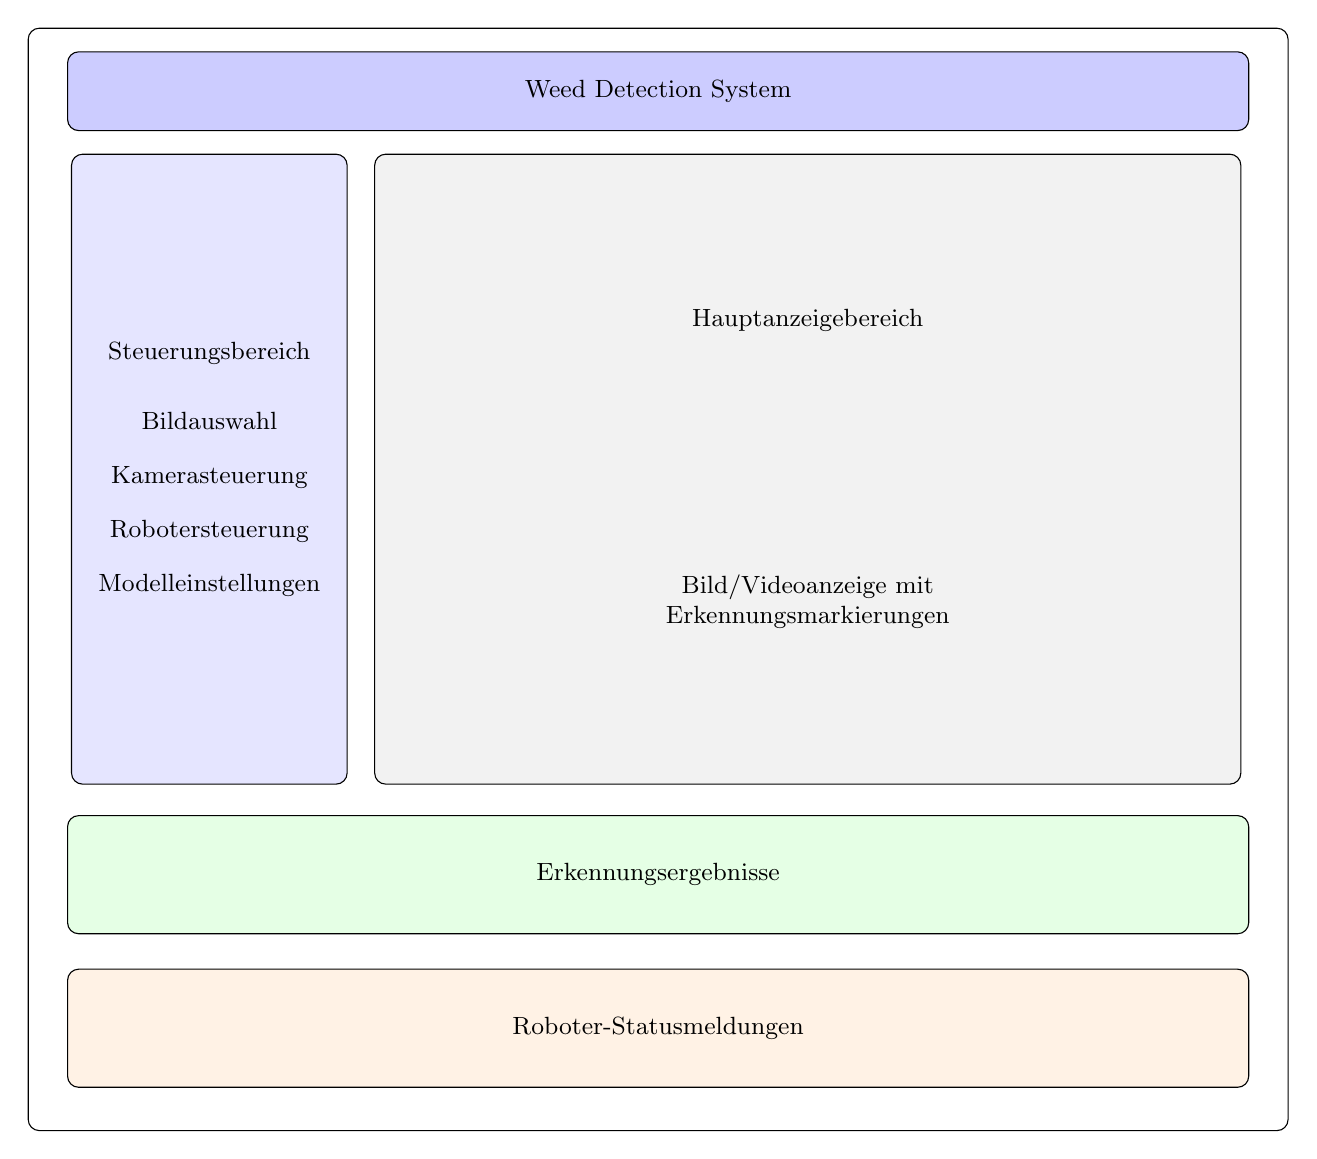
\begin{tikzpicture}[
        scale=1,
        transform shape,
        every node/.style={draw, rounded corners},
        section/.style={rectangle, minimum width=3cm, minimum height=1.5cm, align=center, font=\small}
    ]
    
    % Äußerer Rahmen für das gesamte Fenster
    \node[draw, rectangle, minimum width=16cm, minimum height=14cm, align=center] (window) {};
    
    % Titel
    \node[section, fill=blue!20, minimum width=15cm, minimum height=1cm, align=center] (title) at (0, 6.2) {Weed Detection System};
    
    % Linke Steuerungsleiste
    \node[section, fill=blue!10, minimum width=3.5cm, minimum height=8cm, align=center] (controls) at (-5.7, 1.4) {Steuerungsbereich\\[0.5cm]Bildauswahl\\[0.3cm]Kamerasteuerung\\[0.3cm]Robotersteuerung\\[0.3cm]Modelleinstellungen};
    
    % Hauptbildbereich
    \node[section, fill=gray!10, minimum width=11cm, minimum height=8cm, align=center] (main_display) at (1.9, 1.4) {Hauptanzeigebereich\\[3cm]Bild/Videoanzeige mit\\Erkennungsmarkierungen};
    
    % Ergebnisbereich unten
    \node[section, fill=green!10, minimum width=15cm, minimum height=1.5cm, align=center] (results) at (0, -3.75) {Erkennungsergebnisse};
    
    % Roboter-Statusbereich unten
    \node[section, fill=orange!10, minimum width=15cm, minimum height=1.5cm, align=center] (robot_status) at (0, -5.7) {Roboter-Statusmeldungen};

    \end{tikzpicture}
    \caption{Benutzeroberfläche des WeedDetector-Systems}
    \label{fig:user-interface}
\end{figure}

\newpage

\subsection{Hauptfunktionen}
Die Benutzeroberfläche bietet folgende Hauptfunktionen:

\begin{enumerate}
    \item \textbf{Bildauswahl:} Ermöglicht das Laden eines Bildes aus dem Dateisystem zur Analyse.
    \item \textbf{Kamerasteuerung:} Aktiviert die Echtzeit-Bilderfassung über die angeschlossene Kamera.
    \item \textbf{Robotersteuerung:} Startet und stoppt die automatisierte Unkrauterkennung und -behandlung.
    \item \textbf{Empfindlichkeitseinstellung:} Ermöglicht die Anpassung des Konfidenzwertes für die Erkennung (0,05-0,95).
    \item \textbf{Erkennungsanzeige:} Zeigt erkannte Unkräuter mit Begrenzungsrahmen, Mittelpunktmarkierungen und Beschriftungen an.
    \item \textbf{Ergebnisprotokoll:} Listet detaillierte Informationen zu erkannten Objekten, einschließlich Koordinaten und Konfidenzwerten.
    \item \textbf{Roboterprotokoll:} Dokumentiert alle Aktionen und Statusmeldungen des Robotersystems.
\end{enumerate}

\section{Grundlegende Bedienung}

\subsection{Einzelbildanalyse}
Um ein einzelnes Bild auf Unkraut zu analysieren:
\begin{enumerate}
    \item Klicken Sie auf die Schaltfläche \textbf{"Select Image"}.
    \item Wählen Sie eine Bilddatei aus dem Dateiauswahldialog.
    \item Das System führt automatisch eine Erkennung durch und zeigt die Ergebnisse an.
    \item Passen Sie bei Bedarf den Konfidenzwert an, um die Erkennungsempfindlichkeit zu ändern.
\end{enumerate}

\subsection{Live-Kameraerkennung}
Für die Echtzeit-Unkrauterkennung mit der Kamera:
\begin{enumerate}
    \item Klicken Sie auf die Schaltfläche \textbf{"Start Camera"}.
    \item Die Kamerawird im Hauptanzeigebereich angezeigt.
    \item Erkannte Unkräuter werden in Echtzeit markiert und im Ergebnisbereich aufgelistet.
    \item Zum Beenden der Kameraerkennung klicken Sie auf \textbf{"Stop Camera"}.
\end{enumerate}

\subsection{Robotersteuerung}
Zur Aktivierung des automatisierten Robotermodus:
\begin{enumerate}
    \item Stellen Sie sicher, dass die Kamera aktiviert ist oder aktivieren Sie sie.
    \item Klicken Sie auf die Schaltfläche \textbf{"Start Robot"}.
    \item Der Roboter beginnt mit der automatischen Unkrauterkennung und -behandlung.
    \item Alle Roboterhandlungen werden im Roboter-Statusbereich protokolliert.
    \item Bei Erkennung von Unkraut stoppt der Roboter automatisch
    \item Zum manuellen stoppen des Roboters klicken Sie auf \textbf{"Stop Robot"}.
\end{enumerate}

\section{Erweiterte Funktionen}

\subsection{Anpassung der Erkennungsparameter}
Die Erkennungsgenauigkeit kann durch Anpassung der Confidence konfiguriert werden:
\begin{itemize}
    \item \textbf{Niedriger Confidence-Wert (0,05-0,25):} Erkennt mehr potenzielle Unkräuter, kann aber zu falschen Erkennungen führen.
    \item \textbf{Mittlerer Confidence-Wert (0,25-0,50):} Bietet eine ausgewogene Erkennungsrate für die meisten Anwendungen.
    \item \textbf{Hoher Confidence-Wert (0,50-0,95):} Reduziert Falscherkennungen, kann aber auch tatsächliche Unkräuter übersehen.
\end{itemize}

\subsection{Interpretation der Erkennungsergebnisse}
Die Erkennungsergebnisse werden in folgenden Formaten dargestellt:
\begin{itemize}
    \item \textbf{Visuelle Markierungen:}
    \begin{itemize}
        \item Rote Begrenzungsrahmen um erkannte Unkräuter
        \item Kreuze an den Mittelpunkten der erkannten Objekte
        \item Textbeschriftungen mit Klasse, Koordinaten und Confidence-Wert
    \end{itemize}
    \item \textbf{Ausgabe:}
    \begin{itemize}
        \item Nummerierte Liste erkannter Objekte
        \item Klassenname jedes erkannten Objekts
        \item X/Y-Koordinaten des Mittelpunkts
        \item Confidence-Wert der Erkennung
    \end{itemize}
\end{itemize}

\end{document}
